\documentclass[department=cls, grouplogo=lama, notes={hide notes}, slidesperpage=1, official=true]{beamerruhuisstijl}



\title{Reducing perplexities}
\subtitle{\hspace*{4cm}(and word error rates) \\ \hspace*{6cm} with interpolation factors}
\date{\today}
\author{lama-fan}

\usepackage[backend=bibtex, style=authoryear-comp]{biblatex}
\bibliography{lit}
\usepackage[maxfloats=255]{morefloats}

\usepackage{xparse}
\usepackage{xpatch}

%\hypersetup{colorlinks}% uncomment this line if you prefer colored hyperlinks (e.g., for onscreen viewing)





%\usepackage{etoolbox}
\usepackage{pgfplotstable}
\usepackage{pgfplots}

% patch pgfplots so that \label does the original job
% tufte-book saves the original meaning of \label in
% \@tufte@orig@label
\makeatletter
\patchcmd{\pgfplots@environment@opt}{\label}{\@tufte@orig@label}{}{}
\makeatother

\usepackage{multirow}

\usepackage{makecell}

\usepackage{amsmath}
\usepackage{amssymb}

\usepackage[inline]{enumitem}

\usepackage{tikz}
\usepackage{forest}
\usepackage{subfig} %%% ???

\newcommand{\BON}{\textsf{ngram}\xspace}
\newcommand{\BOL}{\textsf{limited}\xspace}
\newcommand{\BOF}{\textsf{full}\xspace}

\newcommand{\obw}{1bw\xspace}
\renewcommand{\wp}{wp\xspace}
\newcommand{\jrc}{jrc\xspace}
\newcommand{\emea}{emea\xspace}\newcommand{\cgn}{cgn\xspace}
\newcommand{\mediargus}{mediargus\xspace}

\usepackage{graphicx}
%\setkeys{Gin}{width=\linewidth,totalheight=\textheight,keepaspectratio}
%\graphicspath{{graphics/}}

% The fancyvrb package lets us customize the formatting of verbatim
% environments.  We use a slightly smaller font.
\usepackage{fancyvrb}
\fvset{fontsize=\normalsize}


%% use emph in math mode for textnormal
\newcommand{\mathemph}[1]{\textnormal{\emph{#1}}}

% \usepackage{pgfplotstable}
% \usepackage{pgfplots}
\usepackage{environ}
\makeatletter
\newsavebox{\measure@tikzpicture}
\NewEnviron{scaletikzpicturetowidth}[1]{%
  \def\tikz@width{#1}%
  \def\tikzscale{1}\begin{lrbox}{\measure@tikzpicture}%
  \BODY
  \end{lrbox}%
  \pgfmathparse{#1/\wd\measure@tikzpicture}%
  \edef\tikzscale{\pgfmathresult}%
  \BODY
}
\makeatother

% \usetikzlibrary{external}
\pgfplotsset{compat=1.13}
\usepgfplotslibrary{external}
% Enable the library !!!>>> MUST be in the preamble <<<!!!!
\tikzexternalize

\DeclareRobustCommand{\tikzcaption}[1]{\tikzset{external/export next=false}#1}
\DeclareRobustCommand{\tikzref}[1]{\tikzcaption{\ref{#1}}}

\usetikzlibrary{positioning}

\pgfmathsetmacro{\myinnersepp}{2}% inner sep in mm

\tikzset{
box/.style={%draw,%
        inner sep=0,%\myinnersepp,%
        outer sep=0,%
    minimum width=5mm,%
    minimum height=height("Cap")+2*\myinnersepp*1mm,%
    %align=center
    }
}

%%
% Prints an asterisk that takes up no horizontal space.
% Useful in tabular environments.
\newcommand{\hangstar}{\makebox[0pt][l]{*}}

%%
% Prints a trailing space in a smart way.
\usepackage{xspace}

%%
% Some shortcuts for Tufte's book titles.  The lowercase commands will
% produce the initials of the book title in italics.  The all-caps commands
% will print out the full title of the book in italics.
\newcommand{\vdqi}{\textit{VDQI}\xspace}
\newcommand{\ei}{\textit{EI}\xspace}
\newcommand{\ve}{\textit{VE}\xspace}
\newcommand{\be}{\textit{BE}\xspace}
\newcommand{\VDQI}{\textit{The Visual Display of Quantitative Information}\xspace}
\newcommand{\EI}{\textit{Envisioning Information}\xspace}
\newcommand{\VE}{\textit{Visual Explanations}\xspace}
\newcommand{\BE}{\textit{Beautiful Evidence}\xspace}

\newcommand{\TL}{Tufte-\LaTeX\xspace}




% Inserts a blank page
\newcommand{\blankpage}{\newpage\hbox{}\thispagestyle{empty}\newpage}

\usepackage{units}
\usepackage{numprint}

% Typesets the font size, leading, and measure in the form of 10/12x26 pc.
\newcommand{\measure}[3]{#1/#2$\times$\unit[#3]{pc}}

% Macros for typesetting the documentation
\newcommand{\hlred}[1]{\textcolor{Maroon}{#1}}% prints in red
\newcommand{\hangleft}[1]{\makebox[0pt][r]{#1}}
\newcommand{\hairsp}{\hspace{1pt}}% hair space
\newcommand{\hquad}{\hskip0.5em\relax}% half quad space
\newcommand{\TODO}{\textcolor{red}{\bf TODO!}\xspace}
\newcommand{\ie}{\textit{i.\hairsp{}e.}\xspace}
\newcommand{\eg}{\textit{e.\hairsp{}g.}\xspace}
\newcommand{\na}{\quad--}% used in tables for N/A cells
\providecommand{\XeLaTeX}{X\lower.5ex\hbox{\kern-0.15em\reflectbox{E}}\kern-0.1em\LaTeX}
\newcommand{\tXeLaTeX}{\XeLaTeX\index{XeLaTeX@\protect\XeLaTeX}}
% \index{\texttt{\textbackslash xyz}@\hangleft{\texttt{\textbackslash}}\texttt{xyz}}
\newcommand{\tuftebs}{\symbol{'134}}% a backslash in tt type in OT1/T1



\DeclareMathOperator*{\argmin}{arg\,min}
\DeclareMathOperator*{\argmax}{arg\,max}

% Generates the index
\usepackage{makeidx}
\makeindex

%\newcommand{\textcite}[1]{\citet{#1}\cite{#1}}

\usepackage[noabbrev,capitalize]{cleveref}
%\usepackage{backref} 


\usepackage{colortbl}
\definecolor{bestclr}{rgb}{0,0,1}
\definecolor{bestobwclr}{rgb}{1,1,0}
\definecolor{bestjrcclr}{rgb}{0,1,1}
\definecolor{bestemeaclr}{rgb}{1,0,1}
\definecolor{worstclr}{rgb}{1,0,0}
\definecolor{avgclr}{rgb}{1,1,1}
\newcommand{\btc}[1]{\cellcolor{bestclr!#1}}
\newcommand{\wtc}[1]{\cellcolor{worstclr!#1}}

\newcommand{\botc}[1]{\cellcolor{bestobwclr!#1}}
\newcommand{\betc}[1]{\cellcolor{bestjrcclr!#1}}
\newcommand{\bjtc}[1]{\cellcolor{bestemeaclr!#1}}





\usepackage{pgf}
\usepackage{expl3}
\ExplSyntaxOn
\cs_set_eq:NN \eval \fp_eval:n
\ExplSyntaxOff

\usepackage{xintexpr}
\newcommand{\ptc}[1]{% percentage to colour
\ifnum#1>50%
\edef\processme{\noexpand\btc{\eval{round((#1-50)/2)}}}%
    \processme
\else%
\edef\processme{\noexpand\wtc{\eval{round(25-((#1)/2))}}}%
    \processme
\fi%
}

\newcommand{\ptco}[1]{% percentage to colour
	\ifnum#1>50%
	\edef\processme{\cellcolor{bestobwclr!\eval{round((#1-50)/2)}}}%
	\processme
	\else%
	\edef\processme{\noexpand\wtc{\eval{round(25-((#1)/2))}}}%
	\processme
	\fi%
}

\newcommand{\ptcj}[1]{% percentage to colour
	\ifnum#1>50%
	\edef\processme{\cellcolor{bestobwclr!\eval{round((#1-50)/2)}}}%
	\processme
	\else%
	\edef\processme{\noexpand\wtc{\eval{round(25-((#1)/2))}}}%
	\processme
	\fi%
}

\newcommand{\ptce}[1]{% percentage to colour
	\ifnum#1>50%
	\edef\processme{\cellcolor{bestobwclr!\eval{round((#1-50)/2)}}}%
	\processme
	\else%
	\edef\processme{\noexpand\wtc{\eval{round(25-((#1)/2))}}}%
	\processme
	\fi%
}

\usepackage{pgfkeys}
\newcommand{\copr}[3]{% colour & print
%	\ifthenelse{\equal{obw}{#1}}{hoi}{}		\ifthenelse{\equal{jrc}{#1}}{hola}{}
%	\ifthenelse{\equal{emea}{#1}}{he}{}
%\{\pgfkeysvalueof{/#1/min/#2},\pgfkeysvalueof{/#1/max/#2}\}
%\ifdim\pgfkeysvalueof{/#1/min/#2} pt>#3 pt%
%\pgfkeys{/#1/min/#2 = #3}%
%\fi%
%\ifdim\pgfkeysvalueof{/#1/max/#2} pt<#3 pt%
%\pgfkeys{/#1/max/#2 = #3}
%\fi%
\ptc{
\eval{round(100*(((#3-\pgfkeysvalueof{/#1/min/#2}))/(\pgfkeysvalueof{/#1/max/#2}-\pgfkeysvalueof{/#1/min/#2})))}
%\eval{#3}
}%
\numprint{#3}
}

%for a in obw emea jrc; do for b in obw emea jrc wp; do echo "\pgfkeys{/$a/min/$b/.initial="$(grep -o "\\\copr{$a}{$b}{[^ ]\+}" interpolation.tex | sed 's/[^0-9]\+\([0-9.]\+\)}/\1/g' | sort -n | head -n1)"}"; echo "\pgfkeys{/$a/max/$b/.initial="$(grep -o "\\\copr{$a}{$b}{[^ ]\+}" interpolation.tex | sed 's/[^0-9]\+\([0-9.]\+\)}/\1/g' | sort -nr | head -n1)"}"; done; done

\pgfkeys{/obw/min/obw/.initial=114.537}
\pgfkeys{/obw/max/obw/.initial=157.065}
\pgfkeys{/obw/min/emea/.initial=692.109}
\pgfkeys{/obw/max/emea/.initial=1123.89}
\pgfkeys{/obw/min/jrc/.initial=684.972}
\pgfkeys{/obw/max/jrc/.initial=1027.3}
\pgfkeys{/obw/min/wp/.initial=316.727}
\pgfkeys{/obw/max/wp/.initial=555.01}
\pgfkeys{/emea/min/obw/.initial=1211.78}
\pgfkeys{/emea/max/obw/.initial=2007.03}
\pgfkeys{/emea/min/emea/.initial=5.52968}
\pgfkeys{/emea/max/emea/.initial=5.82737}
\pgfkeys{/emea/min/jrc/.initial=650.849}
\pgfkeys{/emea/max/jrc/.initial=1217.94}
\pgfkeys{/emea/min/wp/.initial=653.655}
\pgfkeys{/emea/max/wp/.initial=1329.48}
\pgfkeys{/jrc/min/obw/.initial=1153.54}
\pgfkeys{/jrc/max/obw/.initial=1868.78}
\pgfkeys{/jrc/min/emea/.initial=948.762}
\pgfkeys{/jrc/max/emea/.initial=1475.07}
\pgfkeys{/jrc/min/jrc/.initial=12.4544}
\pgfkeys{/jrc/max/jrc/.initial=14.2414}
\pgfkeys{/jrc/min/wp/.initial=949.004}
\pgfkeys{/jrc/max/wp/.initial=1544.06}

\pgfkeys{/med/min/cr/.initial=441.201} % concat ref 
\pgfkeys{/med/max/cr/.initial=894.406} % concat ref 
\pgfkeys{/med/min/ur/.initial=304.898} % utterance ref
\pgfkeys{/med/max/ur/.initial=660.152} % utterance ref
\pgfkeys{/med/min/cn/.initial=616.996} % concat ngram
\pgfkeys{/med/max/cn/.initial=881.875} % concat ngram
\pgfkeys{/med/min/un/.initial=600.342} % utterance ngram
\pgfkeys{/med/max/un/.initial=677.707} % utterance ngram

\usepackage{array}

\newcolumntype{L}{l<{\hspace{14pt}}}

\renewcommand*\footnoterule{}

\begin{document}

\begin{frame}
    \titlepage
\end{frame}
\note{
}

\begin{frame}{Reducing perplexities and word error rates \\ by improving the interpolation factors \\ of a Bayesian skipgram language model}
    \begin{block}{}
        Louis Onrust \\
        Centre for Language Studies, Radboud University \\
        Center for Processing Speech and Images, KU Leuven
    \end{block}

    \begin{block}{}
        \href{mailto:l.onrust@let.ru.nl}{l.onrust@let.ru.nl} \\
        \href{https://github.com/naiaden}{github.com/naiaden}
    \end{block}
\end{frame}
\note{
}

\begin{frame}{HPYPLMs}
% We apply our language models in Dutch and English to two tasks, namely the intrinsic task of language modelling and the extrinsic task of automatic speech recognition. 
\begin{block}{Hierarchical Pitman-Yor process language model}
\begin{itemize}
    \item Bayesian language model
    \item HPYPLM follows the analogy of the Chinese restaurant process
    \item Generalisation of interpolated Kneser-Ney, which follows the analogy of a soup kitchen
\end{itemize}
\end{block}

\begin{block}{Relevancy}
    \begin{itemize}
        \item As interpolation term for sota language models
        \item First pass decoder ASR
    \end{itemize}
\end{block}

\begin{block}{We report \ldots}
\begin{itemize}
    \item effect of domains in training and testing
    \item perplexities
    \item word error rates
    \end{itemize}
\end{block}
\end{frame}

\begin{frame}{Backoff strategies}
    \begin{block}{ngram}
        Only use the $n$-gram features
    \end{block}

    \begin{block}{full}
        Additionally use skipgrams, full recursively
    \end{block}

    \begin{block}{limited}
        Also skipgrams, but stop if pattern was in training material
    \end{block}
\end{frame}

\begin{frame}{ngram}
\vspace*{-2.2cm}\begin{figure}
    \begin{tikzpicture}[every node/.style={node distance=10pt, rectangle, minimum size=1cm}]
    
    \node[] (d1) {\emph{d}};
    \node[below=of d1] (d2) {\emph{d}};
    \node[below=of d2] (d3) {\emph{d}};
    \node[below=of d3] (d4) {\emph{d}};
    \node[below=of d4] (d5) {\emph{d}};
    \node[below=of d5] (d6) {\emph{d}};
    
    \node[left=0cm and 2.5cm of d1] (axxd1) {\emph{a\{2\}d}};
    \node[left=0cm and 2.5cm of d3] (axxd2) {\emph{a\{2\}d}};
    \node[left=0cm and 2.5cm of d2] (cd1) {\emph{cd}};
    \node[left=0cm and 2.5cm of d5] (cd2) {\emph{cd}};
    \node[left=0cm and 2.5cm of d4] (bxd1) {\emph{b\{1\}d}};
    \node[left=0cm and 2.5cm of d6] (bxd2) {\emph{b\{1\}d}};
    
    \node[left=0cm and 2.5cm of $(axxd1)!0.5!(cd1)$] (axcd) {\emph{a\{1\}cd}};
    \node[left=0cm and 2.5cm of $(axxd2)!0.5!(bxd1)$] (abxd) {\emph{ab\{1\}d}};
    \node[left=0cm and 2.5cm of $(cd2)!0.5!(bxd2)$] (bcd) {\emph{bcd}};
    
    \node[left=0cm and 2.5cm of abxd] (abcd) {\emph{abcd}};
    
    \draw (abcd) -- node[above] {0} ++ (axcd);
    \draw (abcd) -- node[above] {0} ++ (abxd);
    \draw (abcd) -- node[below] {1} ++ (bcd);
    
    \draw (axcd) -- node[above] {0} ++ (axxd1);
    \draw (axcd) -- node[below] {0} ++ (cd1);
    \draw (abxd) -- node[above] {0} ++ (axxd2);
    \draw (abxd) -- node[below] {0} ++ (bxd1);
    \draw (bcd) -- node[above] {1} ++ (cd2);
    \draw (bcd) -- node[below] {0} ++ (bxd2);
    
    \draw (axxd1) -- node[below] {0} ++ (d1);
    \draw (cd1) -- node[below] {0} ++ (d2);
    \draw (axxd2) -- node[below] {0} ++ (d3);
    \draw (bxd1) -- node[below] {0} ++ (d4);
    \draw (cd2) -- node[below] {1} ++ (d5);
    \draw (bxd2) -- node[below] {0} ++ (d6);
   	\end{tikzpicture}
    \label{fig:value}
    \end{figure}
\end{frame}

\begin{frame}{Interpolation factors}
\begin{columns}
\begin{column}{0.5\textwidth}
\begin{block}{uniform}
    All weights are uniformly distributed
\end{block}
\begin{block}{npref}
    Give $n$-grams a higher weight
\end{block}
\begin{block}{value}
    Each backoff step has a specific weight
\end{block}
\begin{block}{count}
    Weights are determined by their context count
\end{block}
\end{column}
\begin{column}{0.5\textwidth}  %%<--- here
\begin{block}{perplexity}
    Weights are determined by their context perplexity
\end{block}
\begin{block}{entropy}
    Weights are determined by their context entropy
\end{block}
\begin{block}{mle}
    Weights are determined by their maximum likelihood estimate
\end{block}
\begin{block}{random}
    Weights are determined randomly
\end{block}
\end{column}
\end{columns}
\end{frame}

\begin{frame}{fulluni}
\vspace*{-2.2cm}\begin{figure}
    \begin{tikzpicture}[every node/.style={node distance=10pt, rectangle, minimum size=1cm}]
    
    \node[] (d1) {\emph{d}};
    \node[below=of d1] (d2) {\emph{d}};
    \node[below=of d2] (d3) {\emph{d}};
    \node[below=of d3] (d4) {\emph{d}};
    \node[below=of d4] (d5) {\emph{d}};
    \node[below=of d5] (d6) {\emph{d}};
    
    \node[left=0cm and 2.5cm of d1] (axxd1) {\emph{a\{2\}d}};
    \node[left=0cm and 2.5cm of d3] (axxd2) {\emph{a\{2\}d}};
    \node[left=0cm and 2.5cm of d2] (cd1) {\emph{cd}};
    \node[left=0cm and 2.5cm of d5] (cd2) {\emph{cd}};
    \node[left=0cm and 2.5cm of d4] (bxd1) {\emph{b\{1\}d}};
    \node[left=0cm and 2.5cm of d6] (bxd2) {\emph{b\{1\}d}};
    
    \node[left=0cm and 2.5cm of $(axxd1)!0.5!(cd1)$] (axcd) {\emph{a\{1\}cd}};
    \node[left=0cm and 2.5cm of $(axxd2)!0.5!(bxd1)$] (abxd) {\emph{ab\{1\}d}};
    \node[left=0cm and 2.5cm of $(cd2)!0.5!(bxd2)$] (bcd) {\emph{bcd}};
    
    \node[left=0cm and 2.5cm of abxd] (abcd) {\emph{abcd}};
    
    \draw (abcd) -- node[above] {1} ++ (axcd);
    \draw (abcd) -- node[above] {1} ++ (abxd);
    \draw (abcd) -- node[below] {1} ++ (bcd);
    
    \draw (axcd) -- node[above] {1} ++ (axxd1);
    \draw (axcd) -- node[below] {1} ++ (cd1);
    \draw (abxd) -- node[above] {1} ++ (axxd2);
    \draw (abxd) -- node[below] {1} ++ (bxd1);
    \draw (bcd) -- node[above] {1} ++ (cd2);
    \draw (bcd) -- node[below] {1} ++ (bxd2);
    
    \draw (axxd1) -- node[below] {1} ++ (d1);
    \draw (cd1) -- node[below] {1} ++ (d2);
    \draw (axxd2) -- node[below] {1} ++ (d3);
    \draw (bxd1) -- node[below] {1} ++ (d4);
    \draw (cd2) -- node[below] {1} ++ (d5);
    \draw (bxd2) -- node[below] {1} ++ (d6);
   	\end{tikzpicture}
    \label{fig:value}
    \end{figure}
\end{frame}

\begin{frame}{Perplexities on English data}
% In the first task, we show that skipgram language models outperform n-gram language models, in and across different text genres, with a large drop in perplexity. 
\npdecimalsign{.}
\nprounddigits{0}
\vspace*{-0.5cm}\begin{table}[]
	\centering
	\label{tab:ngramsvsskipgrams}
	\hspace*{-0.7cm}\begin{tabular}{lllllllllllllll}
		training & \multicolumn{4}{c}{\obw}            &  & \multicolumn{4}{c}{\emea} &  & \multicolumn{4}{c}{\jrc}             \\
		test     & \obw  & \emea  & \jrc  & \wp    
		      &  & \obw  & \emea  & \jrc  & \wp 
		      &  & \obw  & \emea  & \jrc  & \wp      \\ \cline{2-5}\cline{7-10}\cline{12-15}
		\textsf{ngram}   & \copr{obw}{obw}{129.47} &  \copr{obw}{emea}{1123.89} 
					&  \copr{obw}{jrc}{941.4}  &  \copr{obw}{wp}{456.27} &  
		        & \copr{emea}{obw}{1761.34} & \copr{emea}{emea}{5.63033} 
		            & \copr{emea}{jrc}{898} & \copr{emea}{wp}{1123.58} &  
		        &  \copr{jrc}{obw}{1520.1}  &  \copr{jrc}{emea}{1278.94} 
			         &  \copr{jrc}{jrc}{12.85} &  \copr{jrc}{wp}{1249.28} \\
		\textsf{uni}  & \copr{obw}{obw}{124.69} & \copr{obw}{emea}{728.27}  
				 	& \copr{obw}{jrc}{728.98} & \copr{obw}{wp}{392.04} 
				 &  & \copr{emea}{obw}{1393.81} & \copr{emea}{emea}{5.6754} 
				 	& \copr{emea}{jrc}{773.116} & \copr{emea}{wp}{907.558} &  
				 & \copr{jrc}{obw}{1303.66} & \copr{jrc}{emea}{1069.64} 
				 	& \copr{jrc}{jrc}{13.32} & \copr{jrc}{wp}{1067.99} \\
	\end{tabular}
\end{table}
\end{frame}


\begin{frame}{fullnpref}
\vspace*{-2.2cm}\begin{figure}
    \begin{tikzpicture}[every node/.style={node distance=10pt, rectangle, minimum size=1cm}]
    
    \node[] (d1) {\emph{d}};
    \node[below=of d1] (d2) {\emph{d}};
    \node[below=of d2] (d3) {\emph{d}};
    \node[below=of d3] (d4) {\emph{d}};
    \node[below=of d4] (d5) {\emph{d}};
    \node[below=of d5] (d6) {\emph{d}};
    
    \node[left=0cm and 2.5cm of d1] (axxd1) {\emph{a\{2\}d}};
    \node[left=0cm and 2.5cm of d3] (axxd2) {\emph{a\{2\}d}};
    \node[left=0cm and 2.5cm of d2] (cd1) {\emph{cd}};
    \node[left=0cm and 2.5cm of d5] (cd2) {\emph{cd}};
    \node[left=0cm and 2.5cm of d4] (bxd1) {\emph{b\{1\}d}};
    \node[left=0cm and 2.5cm of d6] (bxd2) {\emph{b\{1\}d}};
    
    \node[left=0cm and 2.5cm of $(axxd1)!0.5!(cd1)$] (axcd) {\emph{a\{1\}cd}};
    \node[left=0cm and 2.5cm of $(axxd2)!0.5!(bxd1)$] (abxd) {\emph{ab\{1\}d}};
    \node[left=0cm and 2.5cm of $(cd2)!0.5!(bxd2)$] (bcd) {\emph{bcd}};
    
    \node[left=0cm and 2.5cm of abxd] (abcd) {\emph{abcd}};
    
    \draw (abcd) -- node[above] {$s$} ++ (axcd);
    \draw (abcd) -- node[above] {$s$} ++ (abxd);
    \draw (abcd) -- node[below] {$n$} ++ (bcd);
    
    \draw (axcd) -- node[above] {$s$} ++ (axxd1);
    \draw (axcd) -- node[below] {$n$} ++ (cd1);
    \draw (abxd) -- node[above] {$s$} ++ (axxd2);
    \draw (abxd) -- node[below] {$s$} ++ (bxd1);
    \draw (bcd) -- node[above] {$n$} ++ (cd2);
    \draw (bcd) -- node[below] {$s$} ++ (bxd2);
    
    \draw (axxd1) -- node[below] {$n$} ++ (d1);
    \draw (cd1) -- node[below] {$n$} ++ (d2);
    \draw (axxd2) -- node[below] {$n$} ++ (d3);
    \draw (bxd1) -- node[below] {$n$} ++ (d4);
    \draw (cd2) -- node[below] {$n$} ++ (d5);
    \draw (bxd2) -- node[below] {$n$} ++ (d6);
   	\end{tikzpicture}
    \label{fig:value}
    \end{figure}
\end{frame}

\begin{frame}{Finding the $n$-gram skipgram weight ratio}

\begin{table}\resizebox{\columnwidth}{!}{%
		\begin{tabular}{llllllllllllllllllllllllll}
			\textsf{fullnpref} & 0.0 & 0.1 & 0.1 & 0.1 & 0.1 & 0.2 & 0.2 & 0.3 & 0.4 & 0.5 & 0.6 & 0.8 & 1 & 1.3 & 1.7 & 2.1& 2.7 & 3.5 & 4.5 & 5.7 & 7.4 & 9.4 & 12.1 & 15.6 & 20 \\
			 \obw & \wtc{19.4295700804} & \wtc{17.642782244} & \wtc{14.6752883607} & \wtc{11.2023767913} & \wtc{8.46696959105} & \wtc{6.21740650122} & \wtc{3.19328905977} & \btc{0.045438657812} & \btc{2.85424676686} & \btc{5.52114645229} & \btc{8.27123383432} & \btc{10.6641034603} & \btc{12.8381684726} & \btc{14.7165326809} & \btc{16.3257602237} & \btc{17.5567983223} & \btc{18.4781544914} & \btc{19.0772457183} & \btc{19.38273331} & \btc{19.4295700804} & \btc{19.2590003495} & \btc{18.9171618315} & \btc{18.4445997903} & \btc{17.8818594897} & \btc{17.2645927997} \\
                         \emea & \wtc{19.7839277582} & \wtc{17.6333258196} & \wtc{14.0817274739} & \wtc{9.95820701901} & \wtc{6.74000947645} & \wtc{4.1170801496} & \wtc{0.633565030982} & \btc{3.03234873333} & \btc{6.13979602633} & \btc{9.01194216606} & \btc{11.8682175535} & \btc{14.2343397077} & \btc{16.2455550393} & \btc{17.8203246834} & \btc{18.9673890542} & \btc{19.6067043578} & \btc{19.7839277582} & \btc{19.5042345007} & \btc{18.802701248} & \btc{17.737405753} & \btc{16.3469898473} & \btc{14.7095422323} & \btc{12.8258679461} & \btc{10.8975715449} & \btc{8.84000901643} \\
                         \jrc & \wtc{20.9393339638} & \wtc{18.8263550482} & \wtc{15.30204402} & \wtc{11.1624427185} & \wtc{7.90156503985} & \wtc{5.22577581638} & \wtc{1.647606793} & \btc{2.14955412126} & \btc{5.39688117422} & \btc{8.42774272415} & \btc{11.4793895558} & \btc{14.0498743409} & \btc{16.2861869171} & \btc{18.1019707548} & \btc{19.5143363897} & \btc{20.4275107558} & \btc{20.9017826537} & \btc{20.9393339638} & \btc{20.5781753394} & \btc{19.8758395215} & \btc{18.8791795211} & \btc{17.6627237791} & \btc{16.2760813658} & \btc{14.7856273796} & \btc{13.2386741746} \\
                         \wp & \wtc{20.7199743005} & \wtc{18.7042539314} & \wtc{15.3451526338} & \wtc{11.4047849022} & \wtc{8.2998659864} & \wtc{5.74982180193} & \wtc{2.33296161413} & \btc{1.30671376792} & \btc{4.43607745748} & \btc{7.37767067265} & \btc{10.3692350625} & \btc{12.9246873827} & \btc{15.1911289267} & \btc{17.0848417525} & \btc{18.6278910542} & \btc{19.7157916483} & \btc{20.4145227915} & \btc{20.7199743005} & \btc{20.666541919} & \btc{20.3035478452} & \btc{19.677502047} & \btc{18.8515715502} & \btc{17.8729152989} & \btc{16.7984268815} & \btc{15.6705060825} \\

			
		\end{tabular}
	}
\label{tab:nprefgrid}
\end{table}
\end{frame}

\begin{frame}{Perplexities on English data}
% In the first task, we show that skipgram language models outperform n-gram language models, in and across different text genres, with a large drop in perplexity. 
\npdecimalsign{.}
\nprounddigits{0}
\vspace*{-0.5cm}\begin{table}[]
	\centering
	\label{tab:ngramsvsskipgrams}
	\hspace*{-0.7cm}\begin{tabular}{lllllllllllllll}
		training & \multicolumn{4}{c}{\obw}            &  & \multicolumn{4}{c}{\emea} &  & \multicolumn{4}{c}{\jrc}             \\
		test     & \obw  & \emea  & \jrc  & \wp    
		      &  & \obw  & \emea  & \jrc  & \wp 
		      &  & \obw  & \emea  & \jrc  & \wp      \\ \cline{2-5}\cline{7-10}\cline{12-15}
		\textsf{ngram}   & \copr{obw}{obw}{129.47} &  \copr{obw}{emea}{1123.89} 
					&  \copr{obw}{jrc}{941.4}  &  \copr{obw}{wp}{456.27} &  
		        & \copr{emea}{obw}{1761.34} & \copr{emea}{emea}{5.63033} 
		            & \copr{emea}{jrc}{898} & \copr{emea}{wp}{1123.58} &  
		        &  \copr{jrc}{obw}{1520.1}  &  \copr{jrc}{emea}{1278.94} 
			         &  \copr{jrc}{jrc}{12.85} &  \copr{jrc}{wp}{1249.28} \\
		\textsf{uni}  & \copr{obw}{obw}{124.69} & \copr{obw}{emea}{728.27}  
				 	& \copr{obw}{jrc}{728.98} & \copr{obw}{wp}{392.04} 
				 &  & \copr{emea}{obw}{1393.81} & \copr{emea}{emea}{5.6754} 
				 	& \copr{emea}{jrc}{773.116} & \copr{emea}{wp}{907.558} &  
				 & \copr{jrc}{obw}{1303.66} & \copr{jrc}{emea}{1069.64} 
				 	& \copr{jrc}{jrc}{13.32} & \copr{jrc}{wp}{1067.99} \\ \hline
        \textsf{npref}  & \copr{obw}{obw}{118.28} & \copr{obw}{emea}{699.91}  
		& \copr{obw}{jrc}{694.32} & \copr{obw}{wp}{372.06} 
		&  & \copr{emea}{obw}{1305.9} &  \copr{emea}{emea}{5.59}     
		  & \copr{emea}{jrc}{704.94} & \copr{emea}{wp}{852.52}   &  
		& \copr{jrc}{obw}{1215.52} & \copr{jrc}{emea}{1000.72} 
		& \copr{jrc}{jrc}{12.84} & \copr{jrc}{wp}{1000} \\
	\end{tabular}
\end{table}
\end{frame}


\begin{frame}{Perplexities on English data}
% In the first task, we show that skipgram language models outperform n-gram language models, in and across different text genres, with a large drop in perplexity. 
\npdecimalsign{.}
\nprounddigits{0}
\vspace*{-0.5cm}\begin{table}[]
	\centering
	\label{tab:ngramsvsskipgrams}
	\hspace*{-0.7cm}\begin{tabular}{lllllllllllllll}
		training & \multicolumn{4}{c}{\obw}            &  & \multicolumn{4}{c}{\emea} &  & \multicolumn{4}{c}{\jrc}             \\
		test     & \obw  & \emea  & \jrc  & \wp    
		      &  & \obw  & \emea  & \jrc  & \wp 
		      &  & \obw  & \emea  & \jrc  & \wp      \\ \cline{2-5}\cline{7-10}\cline{12-15}
		\textsf{ngram}   & \copr{obw}{obw}{129.47} &  \copr{obw}{emea}{1123.89} 
					&  \copr{obw}{jrc}{941.4}  &  \copr{obw}{wp}{456.27} &  
		        & \copr{emea}{obw}{1761.34} & \copr{emea}{emea}{5.63033} 
		            & \copr{emea}{jrc}{898} & \copr{emea}{wp}{1123.58} &  
		        &  \copr{jrc}{obw}{1520.1}  &  \copr{jrc}{emea}{1278.94} 
			         &  \copr{jrc}{jrc}{12.85} &  \copr{jrc}{wp}{1249.28} \\
		\textsf{uni}  & \copr{obw}{obw}{124.69} & \copr{obw}{emea}{728.27}  
				 	& \copr{obw}{jrc}{728.98} & \copr{obw}{wp}{392.04} 
				 &  & \copr{emea}{obw}{1393.81} & \copr{emea}{emea}{5.6754} 
				 	& \copr{emea}{jrc}{773.116} & \copr{emea}{wp}{907.558} &  
				 & \copr{jrc}{obw}{1303.66} & \copr{jrc}{emea}{1069.64} 
				 	& \copr{jrc}{jrc}{13.32} & \copr{jrc}{wp}{1067.99} \\ 
        \textsf{npref}  & \copr{obw}{obw}{118.28} & \copr{obw}{emea}{699.91}  
		& \copr{obw}{jrc}{694.32} & \copr{obw}{wp}{372.06} 
		&  & \copr{emea}{obw}{1305.9} &  \copr{emea}{emea}{5.59}     
		  & \copr{emea}{jrc}{704.94} & \copr{emea}{wp}{852.52}   &  
		& \copr{jrc}{obw}{1215.52} & \copr{jrc}{emea}{1000.72} 
		& \copr{jrc}{jrc}{12.84} & \copr{jrc}{wp}{1000} \\ \hline
		\textsf{mle}  & \copr{obw}{obw}{125.17} & \   
				 	& \  & \  
				 &  & \copr{emea}{obw}{1931.25} & \copr{emea}{emea}{5.63} 
				 	& \copr{emea}{jrc}{1015.46} & \copr{emea}{wp}{1225.27} &  
				 & \copr{jrc}{obw}{1535.75} & \copr{jrc}{emea}{1244.74} 
				 	& \  & \  \\
        \textsf{count}  & \copr{obw}{obw}{122.086} & \copr{obw}{emea}{893.166}  
				 	& \copr{obw}{jrc}{885.283} & \copr{obw}{wp}{421.195} 
				 &  & \copr{emea}{obw}{1681.37} & \copr{emea}{emea}{5.61967} 
				 	& \copr{emea}{jrc}{888.956} & \copr{emea}{wp}{1075.4} &  
				 & \copr{jrc}{obw}{1436.12} & \copr{jrc}{emea}{1168.68} 
				 	& \copr{jrc}{jrc}{12.8619} & \copr{jrc}{wp}{1192.74} \\
        \textsf{ent}  & \copr{obw}{obw}{132.26} & \copr{obw}{emea}{794.05}  
				 	& \copr{obw}{jrc}{791.69} & \copr{obw}{wp}{434.24} 
				 &  & \copr{emea}{obw}{1552.49} & \copr{emea}{emea}{5.69} 
				 	& \copr{emea}{jrc}{880.78} & \copr{emea}{wp}{1032.07} &  
				 & \copr{jrc}{obw}{1453.86} & \copr{jrc}{emea}{1179.18} 
				 	& \copr{jrc}{jrc}{13.4475} & \copr{jrc}{wp}{1197.05} \\
        \textsf{ppl}  & \copr{obw}{obw}{157.065} & \copr{obw}{emea}{1002.24}  
				 	& \copr{obw}{jrc}{1027.3} & \copr{obw}{wp}{555.01} 
				 &  & \copr{emea}{obw}{2007.03} & \copr{emea}{emea}{5.82737} 
				 	& \copr{emea}{jrc}{1217.94} & \copr{emea}{wp}{1329.48} &  
				 & \copr{jrc}{obw}{1868.78} & \copr{jrc}{emea}{1475.07} 
				 	& \copr{jrc}{jrc}{14.2414} & \copr{jrc}{wp}{1544.06} \\
	\end{tabular}
\end{table}
\end{frame}


\begin{frame}{fullvalue}
\vspace*{-2.2cm}\begin{figure}
    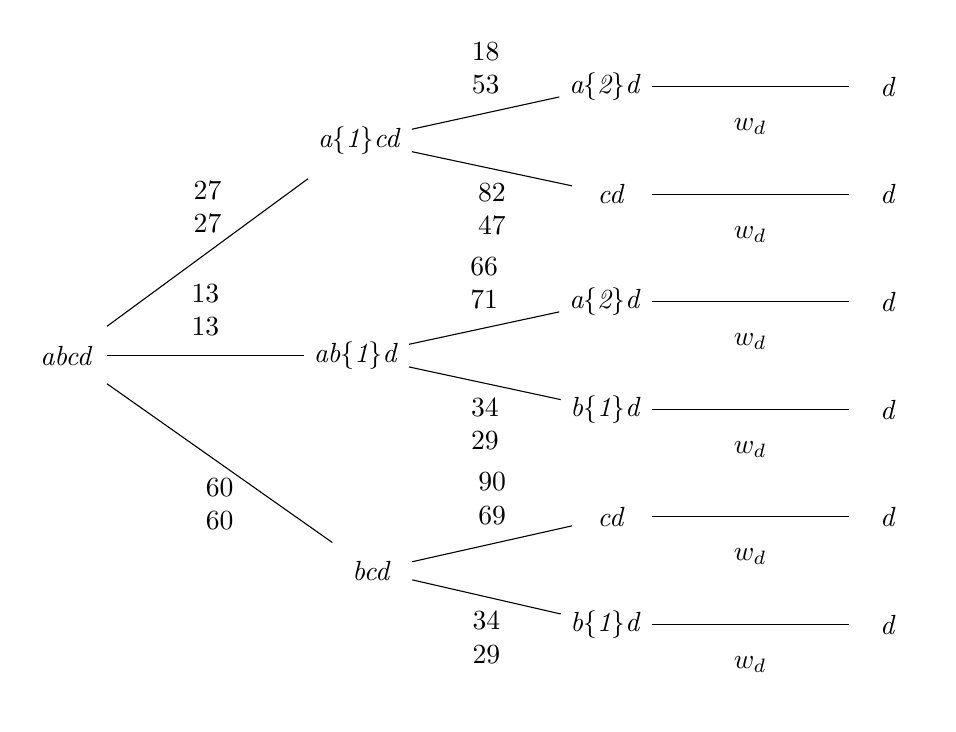
\begin{tikzpicture}[every node/.style={node distance=10pt, rectangle, minimum size=1cm}]
    
    \node[] (d1) {\emph{d}};
    \node[below=of d1] (d2) {\emph{d}};
    \node[below=of d2] (d3) {\emph{d}};
    \node[below=of d3] (d4) {\emph{d}};
    \node[below=of d4] (d5) {\emph{d}};
    \node[below=of d5] (d6) {\emph{d}};
    
    \node[left=0cm and 2.5cm of d1] (axxd1) {\emph{a\{2\}d}};
    \node[left=0cm and 2.5cm of d3] (axxd2) {\emph{a\{2\}d}};
    \node[left=0cm and 2.5cm of d2] (cd1) {\emph{cd}};
    \node[left=0cm and 2.5cm of d5] (cd2) {\emph{cd}};
    \node[left=0cm and 2.5cm of d4] (bxd1) {\emph{b\{1\}d}};
    \node[left=0cm and 2.5cm of d6] (bxd2) {\emph{b\{1\}d}};
    
    \node[left=0cm and 2.5cm of $(axxd1)!0.5!(cd1)$] (axcd) {\emph{a\{1\}cd}};
    \node[left=0cm and 2.5cm of $(axxd2)!0.5!(bxd1)$] (abxd) {\emph{ab\{1\}d}};
    \node[left=0cm and 2.5cm of $(cd2)!0.5!(bxd2)$] (bcd) {\emph{bcd}};
    
    \node[left=0cm and 2.5cm of abxd] (abcd) {\emph{abcd}};
    
    \draw (abcd) -- node[above] {\begin{tabular}{c} 27 \\ 27 \end{tabular}} ++ (axcd);
    \draw (abcd) -- node[above] {\begin{tabular}{c} 13 \\ 13 \end{tabular}} ++ (abxd);
    \draw (abcd) -- node[below] {\begin{tabular}{c} 60 \\ 60 \end{tabular}} ++ (bcd);
    
    \draw (axcd) -- node[above] {\begin{tabular}{c} 18 \\ 53 \end{tabular}} ++ (axxd1);
    \draw (axcd) -- node[below] {\begin{tabular}{c} 82 \\ 47 \end{tabular}} ++ (cd1);
    \draw (abxd) -- node[above] {\begin{tabular}{c} 66 \\ 71 \end{tabular}} ++ (axxd2);
    \draw (abxd) -- node[below] {\begin{tabular}{c} 34 \\ 29 \end{tabular}} ++ (bxd1);
    \draw (bcd) -- node[above] {\begin{tabular}{c} 90 \\ 69 \end{tabular}} ++ (cd2);
    \draw (bcd) -- node[below] {\begin{tabular}{c} 34 \\ 29 \end{tabular}} ++ (bxd2);
    
    \draw (axxd1) -- node[below] {$w_d$} ++ (d1);
    \draw (cd1) -- node[below] {$w_d$} ++ (d2);
    \draw (axxd2) -- node[below] {$w_d$} ++ (d3);
    \draw (bxd1) -- node[below] {$w_d$} ++ (d4);
    \draw (cd2) -- node[below] {$w_d$} ++ (d5);
    \draw (bxd2) -- node[below] {$w_d$} ++ (d6);
   	\end{tikzpicture}
    \label{fig:value}
    \end{figure}
\end{frame}

\begin{frame}{Perplexities on English data}
% In the first task, we show that skipgram language models outperform n-gram language models, in and across different text genres, with a large drop in perplexity. 
\npdecimalsign{.}
\nprounddigits{0}
\vspace*{-0.5cm}\begin{table}[]
	\centering
	\label{tab:ngramsvsskipgrams}
	\hspace*{-0.7cm}\begin{tabular}{lllllllllllllll}
		training & \multicolumn{4}{c}{\obw}            &  & \multicolumn{4}{c}{\emea} &  & \multicolumn{4}{c}{\jrc}             \\
		test     & \obw  & \emea  & \jrc  & \wp    
		      &  & \obw  & \emea  & \jrc  & \wp 
		      &  & \obw  & \emea  & \jrc  & \wp      \\ \cline{2-5}\cline{7-10}\cline{12-15}
		\textsf{ngram}   & \copr{obw}{obw}{129.47} &  \copr{obw}{emea}{1123.89} 
					&  \copr{obw}{jrc}{941.4}  &  \copr{obw}{wp}{456.27} &  
		        & \copr{emea}{obw}{1761.34} & \copr{emea}{emea}{5.63033} 
		            & \copr{emea}{jrc}{898} & \copr{emea}{wp}{1123.58} &  
		        &  \copr{jrc}{obw}{1520.1}  &  \copr{jrc}{emea}{1278.94} 
			         &  \copr{jrc}{jrc}{12.85} &  \copr{jrc}{wp}{1249.28} \\
		\textsf{uni}  & \copr{obw}{obw}{124.69} & \copr{obw}{emea}{728.27}  
				 	& \copr{obw}{jrc}{728.98} & \copr{obw}{wp}{392.04} 
				 &  & \copr{emea}{obw}{1393.81} & \copr{emea}{emea}{5.6754} 
				 	& \copr{emea}{jrc}{773.116} & \copr{emea}{wp}{907.558} &  
				 & \copr{jrc}{obw}{1303.66} & \copr{jrc}{emea}{1069.64} 
				 	& \copr{jrc}{jrc}{13.32} & \copr{jrc}{wp}{1067.99} \\
        \textsf{npref}  & \copr{obw}{obw}{118.28} & \copr{obw}{emea}{699.91}  
		& \copr{obw}{jrc}{694.32} & \copr{obw}{wp}{372.06} 
		&  & \copr{emea}{obw}{1305.9} &  \copr{emea}{emea}{5.59}     
		  & \copr{emea}{jrc}{704.94} & \copr{emea}{wp}{852.52}   &  
		& \copr{jrc}{obw}{1215.52} & \copr{jrc}{emea}{1000.72} 
		& \copr{jrc}{jrc}{12.84} & \copr{jrc}{wp}{1000} \\
		\textsf{mle}  & \copr{obw}{obw}{125.17} & \   
				 	& \  & \  
				 &  & \copr{emea}{obw}{1931.25} & \copr{emea}{emea}{5.63} 
				 	& \copr{emea}{jrc}{1015.46} & \copr{emea}{wp}{1225.27} &  
				 & \copr{jrc}{obw}{1535.75} & \copr{jrc}{emea}{1244.74} 
				 	& \  & \  \\
        \textsf{count}  & \copr{obw}{obw}{122.086} & \copr{obw}{emea}{893.166}  
				 	& \copr{obw}{jrc}{885.283} & \copr{obw}{wp}{421.195} 
				 &  & \copr{emea}{obw}{1681.37} & \copr{emea}{emea}{5.61967} 
				 	& \copr{emea}{jrc}{888.956} & \copr{emea}{wp}{1075.4} &  
				 & \copr{jrc}{obw}{1436.12} & \copr{jrc}{emea}{1168.68} 
				 	& \copr{jrc}{jrc}{12.8619} & \copr{jrc}{wp}{1192.74} \\
        \textsf{ent}  & \copr{obw}{obw}{132.26} & \copr{obw}{emea}{794.05}  
				 	& \copr{obw}{jrc}{791.69} & \copr{obw}{wp}{434.24} 
				 &  & \copr{emea}{obw}{1552.49} & \copr{emea}{emea}{5.69} 
				 	& \copr{emea}{jrc}{880.78} & \copr{emea}{wp}{1032.07} &  
				 & \copr{jrc}{obw}{1453.86} & \copr{jrc}{emea}{1179.18} 
				 	& \copr{jrc}{jrc}{13.4475} & \copr{jrc}{wp}{1197.05} \\
        \textsf{ppl}  & \copr{obw}{obw}{157.065} & \copr{obw}{emea}{1002.24}  
				 	& \copr{obw}{jrc}{1027.3} & \copr{obw}{wp}{555.01} 
				 &  & \copr{emea}{obw}{2007.03} & \copr{emea}{emea}{5.82737} 
				 	& \copr{emea}{jrc}{1217.94} & \copr{emea}{wp}{1329.48} &  
				 & \copr{jrc}{obw}{1868.78} & \copr{jrc}{emea}{1475.07} 
				 	& \copr{jrc}{jrc}{14.2414} & \copr{jrc}{wp}{1544.06} \\ \hline
		\obw-\textsf{value}  & \copr{obw}{obw}{114.537} & \copr{obw}{emea}{712.609}  
				 	& \copr{obw}{jrc}{694.436} & \copr{obw}{wp}{365.706} 
				 &  & \copr{emea}{obw}{1212.13} & \copr{emea}{emea}{5.56569} 
				 	& \copr{emea}{jrc}{655.143} & \copr{emea}{wp}{655.143} &  
				 & \copr{jrc}{obw}{1155.22} & \copr{jrc}{emea}{950.893} 
				 	& \copr{jrc}{jrc}{12.6641} & \copr{jrc}{wp}{949.983} \\
        \emea-\textsf{value}  & \copr{obw}{obw}{115.966} & \copr{obw}{emea}{692.109}  
				 	& \copr{obw}{jrc}{685.726} & \copr{obw}{wp}{366.04} 
				 &  & \copr{emea}{obw}{1221.16} & \copr{emea}{emea}{5.55541} 
				 	& \copr{emea}{jrc}{650.849} & \copr{emea}{wp}{804.805} &  
				 & \copr{jrc}{obw}{1234.75} & \copr{jrc}{emea}{1021.2} 
				 	& \copr{jrc}{jrc}{12.4544} & \copr{jrc}{wp}{1019.34} \\
        \jrc-\textsf{value}  & \copr{obw}{obw}{115.186} & \copr{obw}{emea}{694}  
				 	& \copr{obw}{jrc}{684.972} & \copr{obw}{wp}{364.5} 
				 &  & \copr{emea}{obw}{1372.8} & \copr{emea}{emea}{5.52968} 
				 	& \copr{emea}{jrc}{708.803} & \copr{emea}{wp}{890.016} &  
				 & \copr{jrc}{obw}{1155.73} & \copr{jrc}{emea}{948.762} 
				 	& \copr{jrc}{jrc}{12.6653} & \copr{jrc}{wp}{951.25} \\
        \wp-\textsf{value}  & \copr{obw}{obw}{115.009} & \copr{obw}{emea}{696.297}  
				 	& \copr{obw}{jrc}{685.437} & \copr{obw}{wp}{316.727} 
				 &  & \copr{emea}{obw}{1211.78} & \copr{emea}{emea}{5.56345} 
				 	& \copr{emea}{jrc}{653.655} & \copr{emea}{wp}{653.655} &  
				 & \copr{jrc}{obw}{1153.54} & \copr{jrc}{emea}{950.737} 
				 	& \copr{jrc}{jrc}{12.6445} & \copr{jrc}{wp}{949.004} \\
	\end{tabular}
\end{table}
\end{frame}



\begin{frame}{Perplexities on English data}
% In the first task, we show that skipgram language models outperform n-gram language models, in and across different text genres, with a large drop in perplexity. 
\npdecimalsign{.}
\nprounddigits{0}
\vspace*{-0.5cm}\begin{table}[]
	\centering
	\label{tab:ngramsvsskipgrams}
	\hspace*{-0.7cm}\begin{tabular}{lllllllllllllll}
		training & \multicolumn{4}{c}{\obw}            &  & \multicolumn{4}{c}{\emea} &  & \multicolumn{4}{c}{\jrc}             \\
		test     & \obw  & \emea  & \jrc  & \wp    
		      &  & \obw  & \emea  & \jrc  & \wp 
		      &  & \obw  & \emea  & \jrc  & \wp      \\ \cline{2-5}\cline{7-10}\cline{12-15}
		\textsf{ngram}   & \copr{obw}{obw}{129.47} &  \copr{obw}{emea}{1123.89} 
					&  \copr{obw}{jrc}{941.4}  &  \copr{obw}{wp}{456.27} &  
		        & \copr{emea}{obw}{1761.34} & \copr{emea}{emea}{5.63033} 
		            & \copr{emea}{jrc}{898} & \copr{emea}{wp}{1123.58} &  
		        &  \copr{jrc}{obw}{1520.1}  &  \copr{jrc}{emea}{1278.94} 
			         &  \copr{jrc}{jrc}{12.85} &  \copr{jrc}{wp}{1249.28} \\
		\textsf{uni}  & \copr{obw}{obw}{124.69} & \copr{obw}{emea}{728.27}  
				 	& \copr{obw}{jrc}{728.98} & \copr{obw}{wp}{392.04} 
				 &  & \copr{emea}{obw}{1393.81} & \copr{emea}{emea}{5.6754} 
				 	& \copr{emea}{jrc}{773.116} & \copr{emea}{wp}{907.558} &  
				 & \copr{jrc}{obw}{1303.66} & \copr{jrc}{emea}{1069.64} 
				 	& \copr{jrc}{jrc}{13.32} & \copr{jrc}{wp}{1067.99} \\
        \textsf{npref}  & \copr{obw}{obw}{118.28} & \copr{obw}{emea}{699.91}  
		& \copr{obw}{jrc}{694.32} & \copr{obw}{wp}{372.06} 
		&  & \copr{emea}{obw}{1305.9} &  \copr{emea}{emea}{5.59}     
		  & \copr{emea}{jrc}{704.94} & \copr{emea}{wp}{852.52}   &  
		& \copr{jrc}{obw}{1215.52} & \copr{jrc}{emea}{1000.72} 
		& \copr{jrc}{jrc}{12.84} & \copr{jrc}{wp}{1000} \\
		\textsf{mle}  & \copr{obw}{obw}{125.17} & \   
				 	& \  & \  
				 &  & \copr{emea}{obw}{1931.25} & \copr{emea}{emea}{5.63} 
				 	& \copr{emea}{jrc}{1015.46} & \copr{emea}{wp}{1225.27} &  
				 & \copr{jrc}{obw}{1535.75} & \copr{jrc}{emea}{1244.74} 
				 	& \  & \  \\
        \textsf{count}  & \copr{obw}{obw}{122.086} & \copr{obw}{emea}{893.166}  
				 	& \copr{obw}{jrc}{885.283} & \copr{obw}{wp}{421.195} 
				 &  & \copr{emea}{obw}{1681.37} & \copr{emea}{emea}{5.61967} 
				 	& \copr{emea}{jrc}{888.956} & \copr{emea}{wp}{1075.4} &  
				 & \copr{jrc}{obw}{1436.12} & \copr{jrc}{emea}{1168.68} 
				 	& \copr{jrc}{jrc}{12.8619} & \copr{jrc}{wp}{1192.74} \\
        \textsf{ent}  & \copr{obw}{obw}{132.26} & \copr{obw}{emea}{794.05}  
				 	& \copr{obw}{jrc}{791.69} & \copr{obw}{wp}{434.24} 
				 &  & \copr{emea}{obw}{1552.49} & \copr{emea}{emea}{5.69} 
				 	& \copr{emea}{jrc}{880.78} & \copr{emea}{wp}{1032.07} &  
				 & \copr{jrc}{obw}{1453.86} & \copr{jrc}{emea}{1179.18} 
				 	& \copr{jrc}{jrc}{13.4475} & \copr{jrc}{wp}{1197.05} \\
        \textsf{ppl}  & \copr{obw}{obw}{157.065} & \copr{obw}{emea}{1002.24}  
				 	& \copr{obw}{jrc}{1027.3} & \copr{obw}{wp}{555.01} 
				 &  & \copr{emea}{obw}{2007.03} & \copr{emea}{emea}{5.82737} 
				 	& \copr{emea}{jrc}{1217.94} & \copr{emea}{wp}{1329.48} &  
				 & \copr{jrc}{obw}{1868.78} & \copr{jrc}{emea}{1475.07} 
				 	& \copr{jrc}{jrc}{14.2414} & \copr{jrc}{wp}{1544.06} \\
		\obw-\textsf{value}  & \copr{obw}{obw}{114.537} & \copr{obw}{emea}{712.609}  
				 	& \copr{obw}{jrc}{694.436} & \copr{obw}{wp}{365.706} 
				 &  & \copr{emea}{obw}{1212.13} & \copr{emea}{emea}{5.56569} 
				 	& \copr{emea}{jrc}{655.143} & \copr{emea}{wp}{655.143} &  
				 & \copr{jrc}{obw}{1155.22} & \copr{jrc}{emea}{950.893} 
				 	& \copr{jrc}{jrc}{12.6641} & \copr{jrc}{wp}{949.983} \\
        \emea-\textsf{value}  & \copr{obw}{obw}{115.966} & \copr{obw}{emea}{692.109}  
				 	& \copr{obw}{jrc}{685.726} & \copr{obw}{wp}{366.04} 
				 &  & \copr{emea}{obw}{1221.16} & \copr{emea}{emea}{5.55541} 
				 	& \copr{emea}{jrc}{650.849} & \copr{emea}{wp}{804.805} &  
				 & \copr{jrc}{obw}{1234.75} & \copr{jrc}{emea}{1021.2} 
				 	& \copr{jrc}{jrc}{12.4544} & \copr{jrc}{wp}{1019.34} \\
        \jrc-\textsf{value}  & \copr{obw}{obw}{115.186} & \copr{obw}{emea}{694}  
				 	& \copr{obw}{jrc}{684.972} & \copr{obw}{wp}{364.5} 
				 &  & \copr{emea}{obw}{1372.8} & \copr{emea}{emea}{5.52968} 
				 	& \copr{emea}{jrc}{708.803} & \copr{emea}{wp}{890.016} &  
				 & \copr{jrc}{obw}{1155.73} & \copr{jrc}{emea}{948.762} 
				 	& \copr{jrc}{jrc}{12.6653} & \copr{jrc}{wp}{951.25} \\
        \wp-\textsf{value}  & \copr{obw}{obw}{115.009} & \copr{obw}{emea}{696.297}  
				 	& \copr{obw}{jrc}{685.437} & \copr{obw}{wp}{316.727} 
				 &  & \copr{emea}{obw}{1211.78} & \copr{emea}{emea}{5.56345} 
				 	& \copr{emea}{jrc}{653.655} & \copr{emea}{wp}{653.655} &  
				 & \copr{jrc}{obw}{1153.54} & \copr{jrc}{emea}{950.737} 
				 	& \copr{jrc}{jrc}{12.6445} & \copr{jrc}{wp}{949.004} \\ \hline
	 	\textsf{random}  & \copr{obw}{obw}{129.713} & \copr{obw}{emea}{769.142}  
				 	& \copr{obw}{jrc}{769.019} & \copr{obw}{wp}{411.774} 
				 &  & \copr{emea}{obw}{1483.92} & \copr{emea}{emea}{5.72414} 
				 	& \copr{emea}{jrc}{826.277} & \copr{emea}{wp}{961.939} &  
				 & \copr{jrc}{obw}{1372.32} & \copr{jrc}{emea}{1119.66} 
				 	& \copr{jrc}{jrc}{13.5574} & \copr{jrc}{wp}{1122.53} \\
	\end{tabular}
\end{table}
\end{frame}

\begin{frame}{Perplexities on English data}
% In the first task, we show that skipgram language models outperform n-gram language models, in and across different text genres, with a large drop in perplexity. 
\npdecimalsign{.}
\nprounddigits{0}
\vspace*{-0.5cm}\begin{table}[]
	\centering
	\label{tab:ngramsvsskipgrams}
	\hspace*{-0.7cm}\begin{tabular}{lllllllllllllll}
		training & \multicolumn{4}{c}{\obw}            &  & \multicolumn{4}{c}{\emea} &  & \multicolumn{4}{c}{\jrc}             \\
		test     & \obw  & \emea  & \jrc  & \wp    
		      &  & \obw  & \emea  & \jrc  & \wp 
		      &  & \obw  & \emea  & \jrc  & \wp      \\ \cline{2-5}\cline{7-10}\cline{12-15}
		\textsf{ngram}   & \copr{obw}{obw}{129.47} &  \copr{obw}{emea}{1123.89} 
					&  \copr{obw}{jrc}{941.4}  &  \copr{obw}{wp}{456.27} &  
		        & \copr{emea}{obw}{1761.34} & \copr{emea}{emea}{5.63033} 
		            & \copr{emea}{jrc}{898} & \copr{emea}{wp}{1123.58} &  
		        &  \copr{jrc}{obw}{1520.1}  &  \copr{jrc}{emea}{1278.94} 
			         &  \copr{jrc}{jrc}{12.85} &  \copr{jrc}{wp}{1249.28} \\
	    \textsf{limuni}   & \copr{obw}{obw}{134.17} &  \copr{obw}{emea}{758.54} %limuni done
					&  \copr{obw}{jrc}{755.7}  &  \copr{obw}{wp}{406.31} &  
		        & \copr{emea}{obw}{1421.99} & \copr{emea}{emea}{5.9} 
		            & \copr{emea}{jrc}{793.02} & \copr{emea}{wp}{925.72} &  
		        &  \copr{jrc}{obw}{1353.05}  &  \copr{jrc}{emea}{1112.07} 
			         &  \copr{jrc}{jrc}{14.34} &  \copr{jrc}{wp}{1103.96} \\
	    \textsf{limnpref}   & \copr{obw}{obw}{128.32} &  \copr{obw}{emea}{732.86} %limnpref done
					&  \copr{obw}{jrc}{723.26}  &  \copr{obw}{wp}{387.39} &  
		        & \copr{emea}{obw}{1339.55} & \copr{emea}{emea}{5.83} 
		            & \copr{emea}{jrc}{727.58} & \copr{emea}{wp}{874.17} &  
		        &  \copr{jrc}{obw}{1271.47}  &  \copr{jrc}{emea}{1048.3} 
			         &  \copr{jrc}{jrc}{13.89} &  \copr{jrc}{wp}{1041.44} \\
%		\textsf{limmle}  & \copr{obw}{obw}{138.388} & \copr{obw}{emea}{1027.84}  
%				 	& \copr{obw}{jrc}{993.144} & \copr{obw}{wp}{465.52} 
%				 &  & \copr{emea}{obw}{bbb} & \copr{emea}{emea}{bbb} 
%				 	& \copr{emea}{jrc}{bbb} & \copr{emea}{wp}{bbb} &  
%				 & \copr{jrc}{obw}{ccc} & \copr{jrc}{emea}{ccc} 
%				 	& \copr{jrc}{jrc}{ccc} & \copr{jrc}{wp}{ccc} \\
		\textsf{limcount}   & \copr{obw}{obw}{133.354} &  \copr{obw}{emea}{941.565} 
					&  \copr{obw}{jrc}{927.673}  &  \copr{obw}{wp}{441.112} &  
		        & \copr{emea}{obw}{1745.28} & \copr{emea}{emea}{5.85979} 
		            & \copr{emea}{jrc}{928.113} & \copr{emea}{wp}{1114.12} &  
		        &  \copr{jrc}{obw}{1528.67}  &  \copr{jrc}{emea}{1243.3} 
			         &  \copr{jrc}{jrc}{13.949} &  \copr{jrc}{wp}{1260.12} \\
	    \textsf{liment}   & \copr{obw}{obw}{143.67} &  \copr{obw}{emea}{832.28} 
					&  \copr{obw}{jrc}{824.78}  &  \copr{obw}{wp}{452.52} &  
		        & \copr{emea}{obw}{1583.12} & \copr{emea}{emea}{5.96} 
		            & \copr{emea}{jrc}{903.881} & \copr{emea}{wp}{1052.99} &  
		        &  \copr{jrc}{obw}{1508.13}  &  \copr{jrc}{emea}{1228.23} 
			         &  \copr{jrc}{jrc}{14.6535} &  \copr{jrc}{wp}{1238.09} \\
	    \textsf{limppl}   & \copr{obw}{obw}{172.141} &  \copr{obw}{emea}{1055.32} 
					&  \copr{obw}{jrc}{1074.87}  &  \copr{obw}{wp}{850.723} &  
		        & \copr{emea}{obw}{2049.38} & \copr{emea}{emea}{6.13118} 
		            & \copr{emea}{jrc}{1251.99} & \copr{emea}{wp}{1358.52} &  
		        &  \copr{jrc}{obw}{1945.12}  &  \copr{jrc}{emea}{1543.46} 
			         &  \copr{jrc}{jrc}{15.6463} &  \copr{jrc}{wp}{1602.42} \\
		\textsf{limrandom}  & \copr{obw}{obw}{139.896} & \copr{obw}{emea}{804.404}  
				 	& \copr{obw}{jrc}{799.865} & \copr{obw}{wp}{427.539} 
				 &  & \copr{emea}{obw}{1522.77} & \copr{emea}{emea}{5.95858} 
				 	& \copr{emea}{jrc}{854.708} & \copr{emea}{wp}{985.087} &  
				 & \copr{jrc}{obw}{1433.02} & \copr{jrc}{emea}{1177.73} 
				 	& \copr{jrc}{jrc}{14.611} & \copr{jrc}{wp}{1163.32} \\
	\end{tabular}
\end{table}
\end{frame}


\begin{frame}{Perplexities on Dutch data}
% We confirm this behaviour in a series of experiments in the second task, where we show a reduction in word error rate. Additionally, we show that we can improve over the naive skipgram baseline by some simple heuristics in the form of backoff strategies and interpolation factors.
\npdecimalsign{.}
\nprounddigits{0}
\vspace*{-0.5cm}\begin{table}[]
	\centering
	\label{tab:ngramsvsskipgrams}
	\hspace*{-0.7cm}\begin{tabular}{lllllllllllllll}
		training & \multicolumn{4}{c}{mediargus}   \\
		test     & concat ref  & concat ngram  & utt ref  & utt ngram  \\ \cline{2-5}
		\textsf{srilm}   & \copr{med}{cr}{441.201} &  \copr{med}{cn}{616.996} 
					&  \copr{med}{ur}{660.152}  &  \copr{med}{un}{677.707}  \\
		\textsf{ngram}  & \copr{med}{cr}{894.406} & \copr{med}{cn}{869.218}  
				 	& \copr{med}{ur}{356.52} & \copr{med}{un}{622.422}  \\
        \textsf{fulluni}  & \copr{med}{cr}{723.635} & \copr{med}{cn}{817.861}  
		& \copr{med}{ur}{304.898} & \copr{med}{un}{600.342} \\
		\textsf{limuni}  & \copr{med}{cr}{777.223} & \copr{med}{cn}{881.875}  
		& \copr{med}{ur}{325.777} & \copr{med}{un}{647.464} \\
	\end{tabular}
\end{table}
\end{frame}

\begin{frame}{WER on Dutch data}
\npdecimalsign{.}
\nprounddigits{0}
\vspace*{-0.5cm}\begin{table}[]
	\centering
	\label{tab:ngramsvsskipgrams}
	\hspace*{-0.7cm}\begin{tabular}{lllllllllllllll}
		training & \multicolumn{5}{c}{mediargus}   \\
		test     & concat ref  & concat ngram  & utt ref  & utt ngram & WER \\ \cline{2-5}
		\textsf{srilm}   & \copr{med}{cr}{441.201} &  \copr{med}{cn}{616.996} 
					&  \copr{med}{ur}{660.152}  &  \copr{med}{un}{677.707} & 33.03 \\
		\textsf{ngram}  & \copr{med}{cr}{894.406} & \copr{med}{cn}{869.218}  
				 	& \copr{med}{ur}{356.52} & \copr{med}{un}{622.422} & 32.92 \\
        \textsf{fulluni}  & \copr{med}{cr}{723.635} & \copr{med}{cn}{817.861}  
		& \copr{med}{ur}{304.898} & \copr{med}{un}{600.342} & 34.84 \\
		\textsf{limuni}  & \copr{med}{cr}{777.223} & \copr{med}{cn}{881.875}  
		& \copr{med}{ur}{325.777} & \copr{med}{un}{647.464} & 34.90 \\
	\end{tabular}
\end{table}

\end{frame}

\begin{frame}{}

\end{frame}

\end{document}








    













